\chapter{Kết quả}
\label{chap:results}

Việc đánh giá gồm hai giai đoạn. \textbf{Giai đoạn~1} đo bản thân mô hình trên box ground-truth với che khuất có kiểm soát, theo giao thức đăng ký trước (chọn ngưỡng trên validation, chạy test một lần đã khóa). \textbf{Giai đoạn~2} đo xem lợi thế đó còn lại bao nhiêu khi đặt sau detector YOLOv8n trực tiếp trên che khuất tự nhiên. Mọi số liệu lấy từ các lần chạy test đã đóng băng; khoảng tin cậy (KTC) 95\% là bootstrap ghép cặp trên $15$ địa điểm camera test ($10\,000$ lần rút).

\section{Tiền xử lý Dữ liệu}
\label{sec:data_preprocessing}

Sau khi loại $72\,714$ box nằm trong vùng bỏ qua, còn lại $1\,201\,341$ box phương tiện trong $8\,251$ quỹ đạo. Các tập sự kiện cố định được sinh một lần và băm: $6\,000$ sự kiện validation ($11\,389$ track bị mất) và $12\,000$ sự kiện test ($27\,120$ track bị mất). Mỗi sự kiện gồm $K \le 20$ box cuối của mỗi track bị mất, khoảng trống, histogram màu của track (trung bình trượt hàm mũ) và của mỗi ứng viên (chỉ vùng nhìn thấy), cùng tối đa $8$ xe lân cận tại $t_{\text{lost}}$ và $t_{\text{conf}}$. Tọa độ box được biểu diễn tương đối theo chiều cao box cuối, nên mô hình độc lập với độ phân giải ảnh và khoảng cách tới camera. Vì tập test chính thức có chung $7$ trong $15$ địa điểm camera với train/validation, tập test cũng được chấm riêng trên địa điểm dùng chung và địa điểm chưa thấy: GapLink-Lite đạt lần lượt $93.39\%$ và $93.44\%$ Top-1 (C-3: $80.59\%$ và $79.96\%$), nên hiệu năng không phụ thuộc vào việc đã thấy camera hay chưa.

\section{Phân tích Khám phá Dữ liệu (EDA)}
\label{sec:eda}

Hình~\ref{fig:eda_results} cho thấy phần lớn quỹ đạo ngắn (trung vị $86$ khung hình, $3.4$~s) và giao thông đông (trung bình $8.7$ xe mỗi khung hình; $45\,603$ trong $138\,045$ khung hình có ít nhất mười xe). Giao thông đông đặt các ứng viên trông giống nhau gần xe thật, đây là nguồn chính của liên kết sai, còn quỹ đạo ngắn để lại ít box lịch sử trước khi bị che.

\begin{figure}[H]
    \centering
    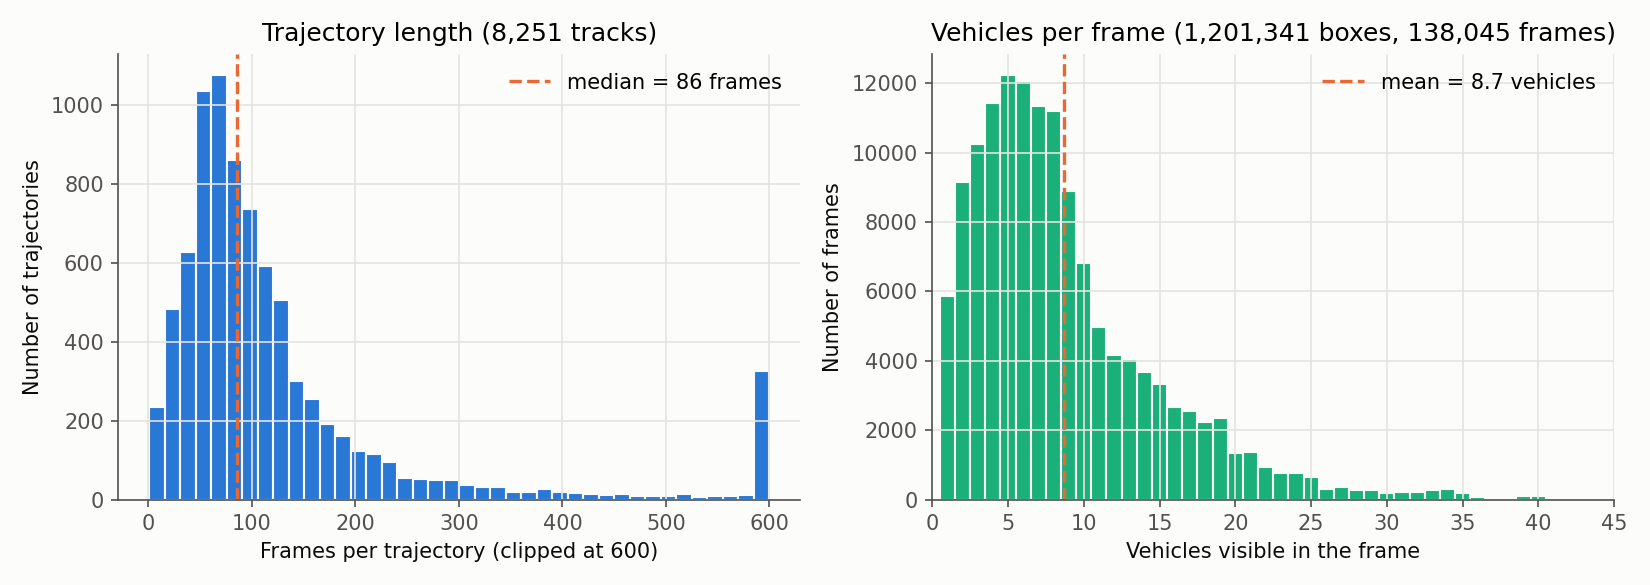
\includegraphics[width=\textwidth]{figures/fig_class_hist.png}
    \caption{Phân tích khám phá dữ liệu: độ dài quỹ đạo (trái) và số xe mỗi khung hình (phải) trên 100 chuỗi đã làm sạch}
    \label{fig:eda_results}
\end{figure}

\section{Mô hình hóa}
\label{sec:modeling}

\subsection{Giai đoạn 1: Đánh giá có Kiểm soát trên Box Ground-Truth}
\label{sec:phase1}

\textbf{Tái liên kết cấp sự kiện.} Bảng~\ref{tab:event_results} so sánh checkpoint đã đóng băng với ba baseline cổ điển tại ngưỡng chọn trên validation. GapLink-Lite đạt $\mathbf{93.41\%}$ Top-1 với $\mathbf{3.01\%}$ liên kết sai (trung bình 5 seed $93.64\% \pm 0.14\%$), so với $80.29\%$ / $19.24\%$ của baseline Kalman C-3 và $83.69\%$ / $15.88\%$ của baseline mạnh nhất C-4. Mức tăng là $+13.12$~pp so với C-3 (KTC $[12.29, 14.19]$) và $+9.72$~pp so với C-4 ($[8.68, 10.94]$), và lớn nhất ở nơi mô hình chuyển động cổ điển thất bại: với khoảng trống dài ($46$--$90$ khung hình), Top-1 tăng từ $64.24\%$ (C-4) lên $79.58\%$. Hình~\ref{fig:wlr_curve} cho thấy đây không phải hệ quả của việc chọn ngưỡng: trên toàn dải ngưỡng, đường của GapLink-Lite nằm trên mọi đường baseline.

\begin{table}[H]
    \centering
    \caption{Giai đoạn 1 --- tái liên kết cấp sự kiện trên tập test đã khóa ($12\,000$ sự kiện, $27\,120$ track bị mất). Mọi ngưỡng chọn trên validation.}
    \label{tab:event_results}
    \scriptsize\setlength{\tabcolsep}{2.8pt}
    \begin{tabularx}{\textwidth}{X c c c c c c c}
        \toprule
        \textbf{Phương pháp (điểm vận hành)} & \textbf{Top-1 (\%)} & \textbf{Ngắn} & \textbf{TB} & \textbf{Dài} & \textbf{Khó (\%)} & \textbf{Dust F1} & \textbf{WLR (\%)} \\
        \midrule
        C-2 (Top-1 val tốt nhất) & 76.58 & 87.80 & 76.64 & 49.10 & 77.73 & 44.77 & 21.14 \\
        C-3 (Top-1 val tốt nhất) & 80.29 & 94.23 & 76.74 & 54.39 & 81.70 & 52.31 & 19.24 \\
        C-4 (Top-1 val tốt nhất) & 83.69 & 94.41 & 80.77 & 64.24 & 85.85 & 51.22 & 15.88 \\
        \midrule
        C-2 (Val WLR$\le$5\%) & 70.59 & 93.82 & 63.88 & 29.32 & 69.67 & 49.41 & 6.46 \\
        C-3 (Val WLR$\le$5\%, $\theta=0.5$) & 57.22 & 46.68 & 68.79 & 56.54 & 55.76 & 39.40 & 9.13 \\
        C-4 (Val WLR$\le$5\%) & 76.03 & 74.02 & 82.25 & 66.79 & 75.89 & 54.01 & 6.70 \\
        \midrule
        \textbf{GapLink-Lite (Seed 1)} & \textbf{93.41} & \textbf{98.64} & \textbf{93.89} & \textbf{79.58} & \textbf{93.18} & \textbf{83.97} & \textbf{3.01} \\
        \textbf{GapLink-Lite (TB 5 seed)} & \textbf{93.64} & \textbf{98.46} & \textbf{94.17} & \textbf{80.67} & \textbf{93.47} & \textbf{84.61} & \textbf{2.98} \\
        \bottomrule
    \end{tabularx}
\end{table}

\begin{figure}[H]
    \centering
    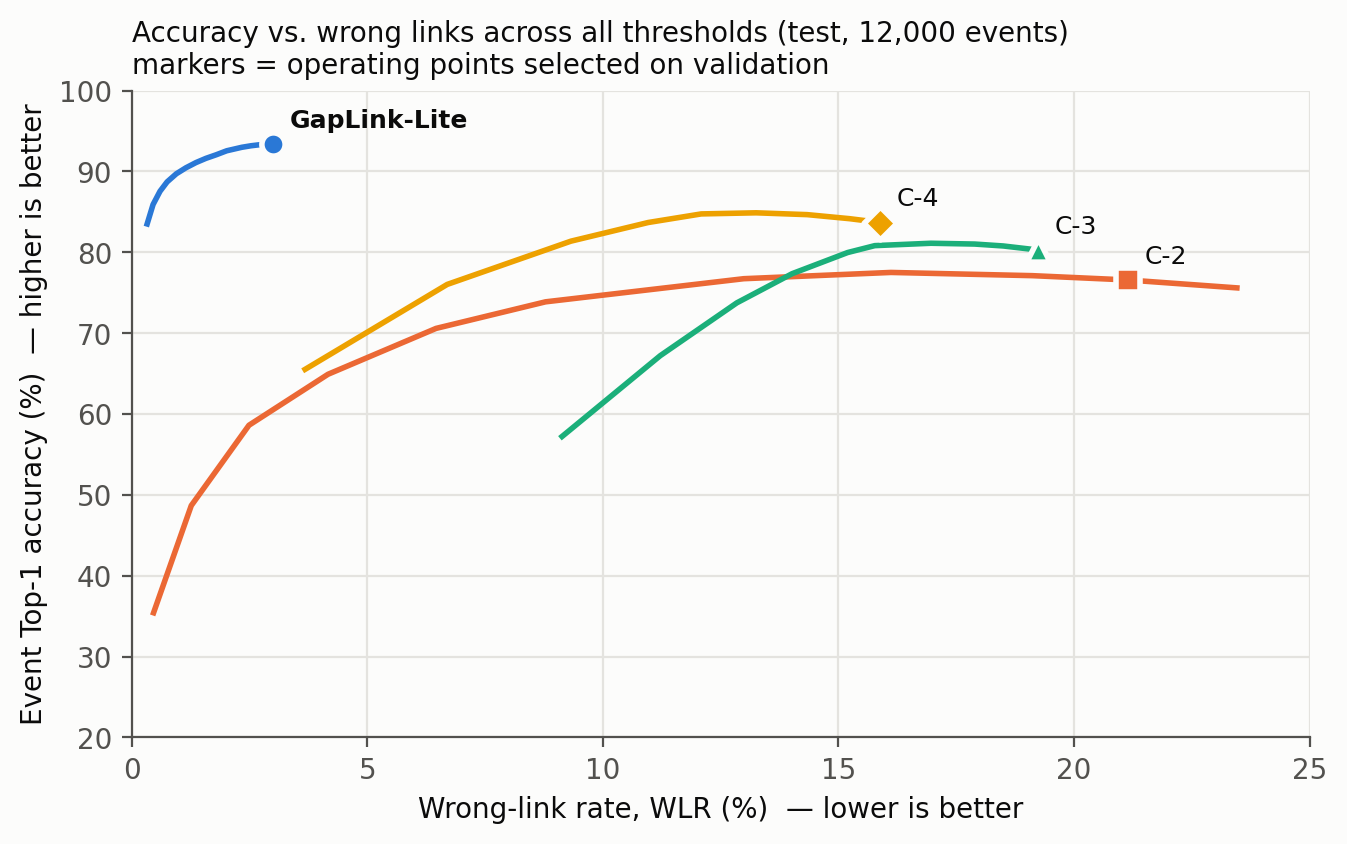
\includegraphics[width=0.86\textwidth]{figures/fig_top1_vs_wlr_curve.png}
    \caption{Top-1 cấp sự kiện theo tỉ lệ liên kết sai trên toàn dải ngưỡng (test). Điểm đánh dấu: điểm vận hành chọn trên validation.}
    \label{fig:wlr_curve}
\end{figure}

\textbf{Hiệu chuẩn độ bất định (H2).} Tiêu chí đăng ký trước yêu cầu độ phủ 90\% sau hiệu chuẩn nằm trong $[85, 95]\%$ ở cả ba nhóm khoảng trống. Khoảng trống ngắn và trung bình đạt, nhưng nhóm khoảng trống dài phủ hơi quá ($95.14\%$ trên validation, $95.86\%$ trên test), nên \textbf{H2 không được ủng hộ}; hệ số tỉ lệ cho khoảng trống dài chỉ được khớp trên bốn địa điểm validation. Đầu Gaussian thô vốn đã gần hiệu chuẩn (test: $86.42\% / 85.46\% / 88.02\%$ cho khoảng trống ngắn/trung bình/dài) và sắc hơn nhiều so với baseline Kalman, có ellipse phủ quá ở mức khoảng $98\%$ với NLL cao hơn ($9.15$ so với $7.99$); đây là quan sát hậu kiểm, không phải giả thuyết đạt.

\textbf{Tracking trực tuyến (H3, P1).} Trong tracker trực tuyến hai tầng (Bảng~\ref{tab:tracker_results}), GapLink-Lite khôi phục $\mathbf{96.20\%}$ che khuất được chèn với chỉ $\mathbf{0.21\%}$ liên kết sai, so với $85.17\%$ / $4.32\%$ của C-2 và $84.96\%$ / $10.25\%$ của C-3; IDF1 tăng từ $77.60\%$ (C-3) lên $\mathbf{99.11\%}$ và số lần đổi danh tính giảm từ $342$ xuống $98$. Mức tăng IRR so với C-3 là $+11.24$~pp (KTC $[9.10, 14.35]$), và GapLink-Lite vượt cả C-2 lẫn C-3 ở cả ba nhóm khoảng trống, nên \textbf{H3 được ủng hộ}. Khi che khuất một phần và chỉ dùng ngoại hình vùng nhìn thấy, kết quả vẫn giữ ($95.99\%$ IRR, $0.36\%$ WLR). Kiểm tra giao thức \textbf{P1 đạt}: khi không tái liên kết (C-1), IRR là $0.00\%$.

\begin{table}[H]
    \centering
    \caption{Giai đoạn 1 --- tracker trực tuyến trên $40$ chuỗi test ($1\,922$ khoảng che khuất được chèn, $a_{\max}=95$)}
    \label{tab:tracker_results}
    \resizebox{\textwidth}{!}{%
    \begin{tabular}{@{}l rrrrrrrrr@{}}
        \toprule
        \textbf{Tracker} & \shortstack{\textbf{Toàn}\\\textbf{IRR}} & \shortstack{\textbf{Toàn}\\\textbf{WLR}} & \shortstack{\textbf{Toàn}\\\textbf{IDF1}} & \shortstack{\textbf{Toàn}\\\textbf{MOTA}} & \shortstack{\textbf{Toàn}\\\textbf{IDSW}} & \shortstack{\textbf{Phần}\\\textbf{IRR}} & \shortstack{\textbf{Phần}\\\textbf{WLR}} & \shortstack{\textbf{Phần}\\\textbf{IDF1}} & \shortstack{\textbf{Phần}\\\textbf{IDSW}} \\
        \midrule
        C-1 (chỉ IoU) & 0.00 & 0.00 & 74.18 & 99.59 & 2127 & 0.00 & 0.00 & 74.18 & 2127 \\
        C-2 (Const-Vel) & 85.17 & 4.32 & 94.66 & 99.92 & 331 & 85.38 & 4.21 & 94.42 & 327 \\
        C-3 (Kalman) & 84.96 & 10.25 & 77.60 & 99.93 & 342 & 81.17 & 14.15 & 76.63 & 416 \\
        C-3 (WLR$\le$5\%) & 77.58 & 3.07 & 95.23 & 99.88 & 487 & 49.43 & 7.70 & 87.21 & 1029 \\
        C-4 (C-3+S+C) & 85.12 & 10.15 & 76.98 & 99.93 & 338 & 82.21 & 12.90 & 76.43 & 395 \\
        \textbf{GapLink-Lite} & \textbf{96.20} & \textbf{0.21} & \textbf{99.11} & \textbf{99.98} & \textbf{98} & \textbf{95.99} & \textbf{0.36} & \textbf{99.02} & \textbf{103} \\
        \bottomrule
    \end{tabular}%
    }
\end{table}

\subsection{Giai đoạn 2: Ứng dụng với Detector YOLOv8n Trực tiếp}
\label{sec:phase2}

\textbf{Thiết lập.} Mọi phương pháp nhận cùng detection YOLOv8n (kích thước đầu vào $640$, ngưỡng tin cậy $0.28$) và dùng chung tracker tầng 1, cửa sổ track bị mất ($a_{\max}=95$) và quy tắc an ninh; chỉ module tái liên kết khác nhau. Ground truth chỉ được dùng sau đó để chấm điểm. Với mọi phương pháp, ngưỡng chấp nhận được chọn trên $13$ video validation theo cùng một quy tắc (Nat-IRR cao nhất với điều kiện Nat-WLR $\le 5\%$) và đánh giá một lần trên $40$ video test. GapLink-Lite dùng checkpoint thích ứng detector v1.3 (Mục~\ref{sec:training_process}).

\textbf{Kết quả.} Bảng~\ref{tab:live_v13} và Hình~\ref{fig:live_scatter} cho thấy kết quả. So với họ Kalman làm nền cho các tracker công nghiệp, GapLink-Lite tốt hơn trên cả hai trục: Nat-IRR $\mathbf{84.41\%}$ so với $57.63\%$ (C-3) và $61.85\%$ (C-4), Nat-WLR $\mathbf{6.09\%}$ so với $24.70\%$ và $9.94\%$. So với baseline mạnh nhất là vận tốc không đổi (C-2), khả năng khôi phục ngang nhau ($84.41\%$ so với $84.58\%$; $\Delta = -0.17$~pp, KTC $[-1.33, 1.08]$) trong khi \textbf{liên kết sai giảm một nửa} ($6.09\%$ so với $12.92\%$; $\Delta = -6.82$~pp, KTC $[-11.04, -3.18]$). Về số tuyệt đối, GapLink-Lite có $313$ tái liên kết sai trên $5\,137$, so với $676$ trên $5\,234$ của C-2 và $1\,072$ trên $4\,340$ của C-3. Trong bảng điều khiển an ninh, một liên kết sai là một báo động giả, và GapLink-Lite cũng có tỉ lệ báo động giả lộ trình cấm thấp nhất ($9.27\%$, tức $14$ cảnh báo giả so với $18$ của C-2 và $70$ của C-3). Cái giá của sự thận trọng này là recall lộ trình: nó bắt được $69$ trên $162$ vi phạm bị che với đúng ID, so với $77$ của C-3 và $80$ của C-4. Checkpoint thích ứng detector là yếu tố làm điều này khả thi: với checkpoint gốc, tỉ lệ liên kết sai trực tiếp là $10.20\%$, và fine-tune giảm $4.11$~pp (KTC $[1.57, 5.98]$) với cái giá $2.89$~pp khả năng khôi phục. Trên validation, C-2 dẫn $4$~pp Nat-IRR; thứ hạng này không giữ nguyên trên test, cho thấy bốn địa điểm validation khiến việc chọn điểm vận hành có nhiều nhiễu.

\begin{table}[H]
    \centering
    \caption{Giai đoạn 2 --- đánh giá YOLOv8n trực tiếp với điểm vận hành chọn trên validation. Validation: $13$ video; test: $40$ video. Độ đo lộ trình trên các lượt đi $Z_A\!\to\!Z_B$ có che khuất. $^\dagger$không ngưỡng nào đạt Nat-WLR $\le 5\%$ trên validation (dùng quy tắc WLR thấp nhất).}
    \label{tab:live_v13}
    \resizebox{\textwidth}{!}{%
    \begin{tabular}{@{}l rr rr rr@{}}
        \toprule
        & \multicolumn{2}{c}{\textbf{Validation}} & \multicolumn{4}{c}{\textbf{Test}} \\
        \cmidrule(lr){2-3}\cmidrule(lr){4-7}
        \textbf{Phương pháp (điểm vận hành)} & \textbf{Nat-IRR} & \textbf{Nat-WLR} & \textbf{Nat-IRR} & \textbf{Nat-WLR} & \textbf{Lộ trình rec.} & \textbf{Lộ trình FAR} \\
        \midrule
        C-1 (chỉ IoU) & 6.05 & 0.00 & 8.93 & 0.00 & 33.33 & 3.45 \\
        C-2 ($\theta=1.2$) & \textbf{81.56} & 4.87 & \textbf{84.58} & 12.92 & 41.98 & 11.32 \\
        C-3 ($\theta=1.0$)$^\dagger$ & 32.23 & 16.37 & 57.63 & 24.70 & 47.53 & 32.56 \\
        C-4 ($\theta=1.2$) & 32.08 & \textbf{3.81} & 61.85 & 9.94 & \textbf{49.38} & 14.04 \\
        GapLink-Lite v1.1 ($\tau=0.25$, tham chiếu) & 81.69 & 13.33 & 87.30 & 10.20 & 45.68 & 12.88 \\
        \textbf{GapLink-Lite v1.3} ($\tau=0.65$) & 77.55 & 4.21 & 84.41 & \textbf{6.09} & 42.59 & \textbf{9.27} \\
        \bottomrule
    \end{tabular}%
    }
\end{table}

\begin{figure}[H]
    \centering
    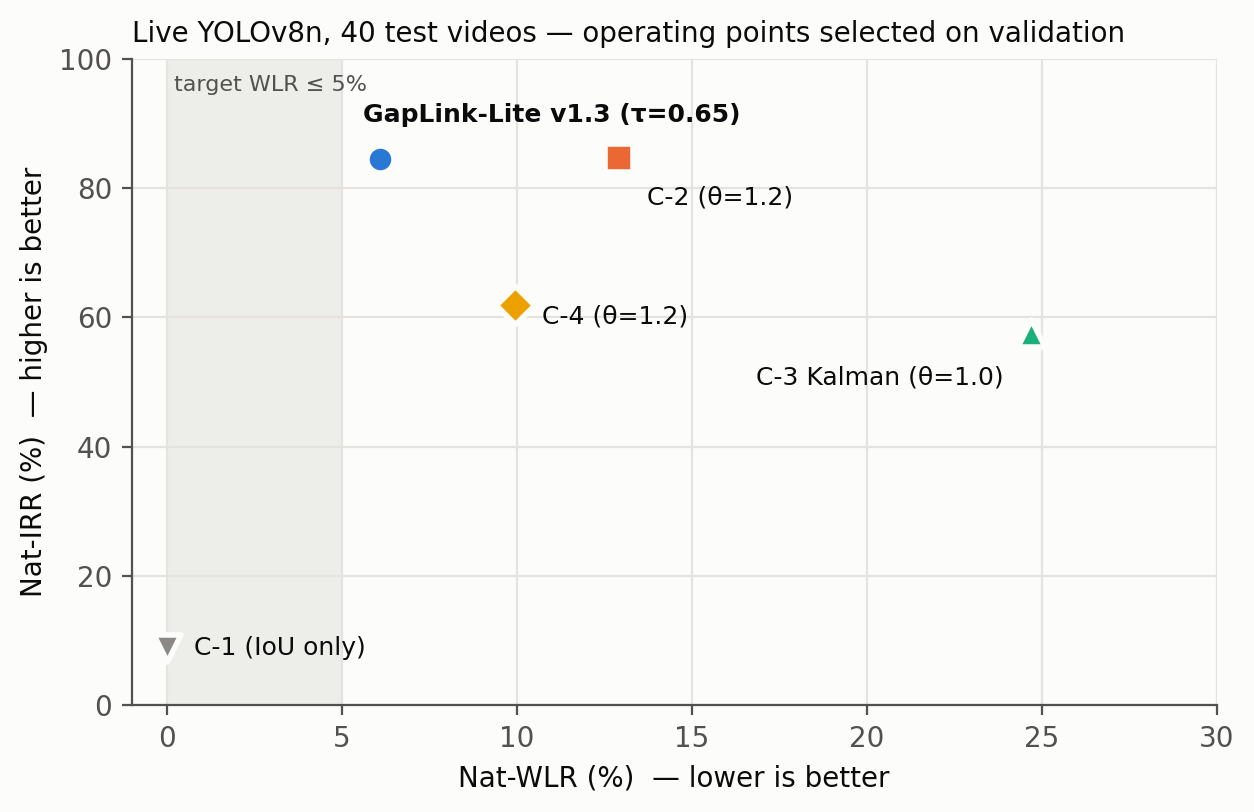
\includegraphics[width=0.78\textwidth]{figures/fig_live_v13_scatter.png}
    \caption{Giai đoạn 2 --- khôi phục so với liên kết sai trên $40$ video test trực tiếp (điểm vận hành chọn trên validation).}
    \label{fig:live_scatter}
\end{figure}

\textbf{Thời gian xử lý với detector trực tiếp.} Một phiên bản trước của bảng điều khiển (mô hình chạy trên GPU) đã được profile trên clip nút giao đông nhất với YOLOv8n chạy trực tiếp: $28.95$~ms mỗi khung hình ($34.5$~FPS), gồm $12.53$~ms cho YOLOv8n, $3.26$~ms cho histogram và lọc box, và $13.16$~ms cho tracking, quy tắc và vẽ. Bảng điều khiển cuối dùng detection đã cache và mô hình trên CPU; thời gian của nó với detector trực tiếp chưa được đo lại.

\subsection{Phân tích Lỗi, Ablation và Độ bền}
\label{sec:error_analysis}

\textbf{Các phương pháp sai như thế nào.} Bảng~\ref{tab:error_taxonomy} phân loại toàn bộ $27\,120$ track bị mất trong tập test. Hai cách tiếp cận sai theo hai hướng ngược nhau. Baseline Kalman gần như không bao giờ từ chối; lỗi của nó là liên kết với xe sai ($32.2\%$ track khoảng trống dài) hoặc với một xe mới sau khi xe thật đã rời đi ($13.3\%$). Lỗi chủ yếu của GapLink-Lite ở khoảng trống dài là lỗi thận trọng --- từ chối tái liên kết ($10.4\%$), để lại quỹ đạo bị tách nhưng đúng --- trong khi liên kết sai và liên kết giả chỉ ở mức $7.4\%$ và $2.6\%$. Với giám sát, nơi một liên kết sai trở thành báo động giả hoặc mục tiêu bị cướp, kiểu lỗi này an toàn hơn. Mười sự kiện test có xác suất thấp nhất cho đáp án đúng thực sự mơ hồ: xe thật xuất hiện lại xa đường ngoại suy sau khi dừng hoặc rẽ, hoặc cạnh một xe trông giống; baseline Kalman sai cả mười ca.

\begin{table}[H]
    \centering
    \caption{Kết cục của mọi track bị mất trong tập test theo nhóm khoảng trống (\% số track trong nhóm)}
    \label{tab:error_taxonomy}
    \small
    \begin{tabular}{@{}l l r r r r@{}}
        \toprule
        \textbf{Phương pháp} & \textbf{Nhóm khoảng trống} & \textbf{Đúng} & \textbf{Bỏ lỡ} & \textbf{Sai xe} & \textbf{Liên kết sau khi rời}  \\
        \midrule
        C-3 (Kalman) & Ngắn (3--15) & 94.2 & 0.8 & 1.4 & 3.6 \\
        C-3 (Kalman) & Trung bình (16--45) & 76.7 & 0.3 & 11.4 & 11.5 \\
        C-3 (Kalman) & Dài (46--90) & 54.4 & 0.1 & 32.2 & 13.3 \\
        \midrule
        GapLink-Lite & Ngắn (3--15) & 98.6 & 0.8 & 0.2 & 0.3 \\
        GapLink-Lite & Trung bình (16--45) & 93.9 & 3.5 & 1.3 & 1.3 \\
        GapLink-Lite & Dài (46--90) & 79.6 & 10.4 & 7.4 & 2.6 \\
        \bottomrule
    \end{tabular}
\end{table}

\textbf{Tính nhất quán giữa các camera.} GapLink-Lite có Top-1 cấp sự kiện và IRR tracker cao nhất ở \textbf{cả $15$ địa điểm test}, kể cả $8$ địa điểm chưa từng thấy khi huấn luyện; điểm thấp nhất theo địa điểm của nó ($89.7\%$ Top-1) vẫn cao hơn điểm cao nhất theo địa điểm của C-3 ($86.8\%$).

\textbf{Ablation và độ bền.} Bảng~\ref{tab:ablation_results} lần lượt bỏ từng thành phần (mỗi biến thể 5 seed). Điều kiện hóa theo khoảng trống quan trọng nhất ($-3.66 \pm 0.12$~pp tổng thể, $-8.91$~pp với khoảng trống dài), tiếp theo là histogram màu ($-2.20 \pm 0.26$~pp); ngữ cảnh xe lân cận DeepSets không cho mức tăng đáng tin cậy về mặt thống kê trên benchmark này ($-0.50 \pm 0.74$~pp). Khi gây nhiễu tập sự kiện test, GapLink-Lite giữ tỉ lệ liên kết sai dưới $6\%$ khi nhiễu vị trí tới $8\times$ và mất $30\%$ ứng viên đúng, trong những điều kiện mà tỉ lệ liên kết sai của C-3 tăng lên $28$--$35\%$.

\begin{table}[H]
    \centering
    \caption{Ablation có kiểm soát 5 seed trên tập test đã khóa ($12\,000$ sự kiện, trung bình $\pm$ độ lệch chuẩn qua 5 seed)}
    \label{tab:ablation_results}
    \small\setlength{\tabcolsep}{3.0pt}
    \begin{tabularx}{\textwidth}{X c c c c c}
        \toprule
        \textbf{Biến thể (5 seed)} & \textbf{Top-1 (\%)} & \textbf{Khoảng dài (\%)} & \textbf{Dust.\ F1 (\%)} & \textbf{WLR (\%)} & \textbf{$\Delta$ Top-1 (pp)} \\
        \midrule
        \textbf{Mô hình đầy đủ} & $\mathbf{93.64\pm0.14}$ & $\mathbf{80.67\pm0.82}$ & $\mathbf{84.61}$ & $\mathbf{2.98}$ & --- \\
        bỏ ngữ cảnh & $93.14\pm0.61$ & $78.60\pm1.41$ & 84.01 & 3.80 & $-0.50\pm0.74$ \\
        bỏ màu & $91.44\pm0.24$ & $72.72\pm0.99$ & 82.11 & 5.14 & $-2.20\pm0.26$ \\
        không biết khoảng trống ($g$ cố định) & $89.98\pm0.09$ & $71.76\pm0.35$ & 77.61 & 5.05 & $-3.66\pm0.12$ \\
        \bottomrule
    \end{tabularx}
\end{table}

\section{Giao diện Người dùng}
\label{sec:user_interface}

\textbf{GapLink-VMS} là bảng điều khiển web cục bộ phát một clip và hiển thị song song tracker baseline (C-3 Kalman, bên trái) và GapLink-Lite v1.3 (bên phải) trên cùng detection YOLOv8n (Hình~\ref{fig:vms_ui}). Giao diện được chủ động tối giản, chỉ giữ những gì buổi trình diễn cần: ba nút chọn clip, phát/tạm dừng, chạy từng khung hình, thanh tua, tốc độ phát ($1\times$, $0.5\times$, $0.25\times$), công tắc bật/tắt ID, công cụ vẽ vùng cho clip lộ trình và click để khóa cho clip mục tiêu. Cột bên phải hiển thị bảng kết quả của clip hiện tại và lịch sử sự cố với ảnh cắt trước/sau.

\begin{figure}[H]
    \centering
    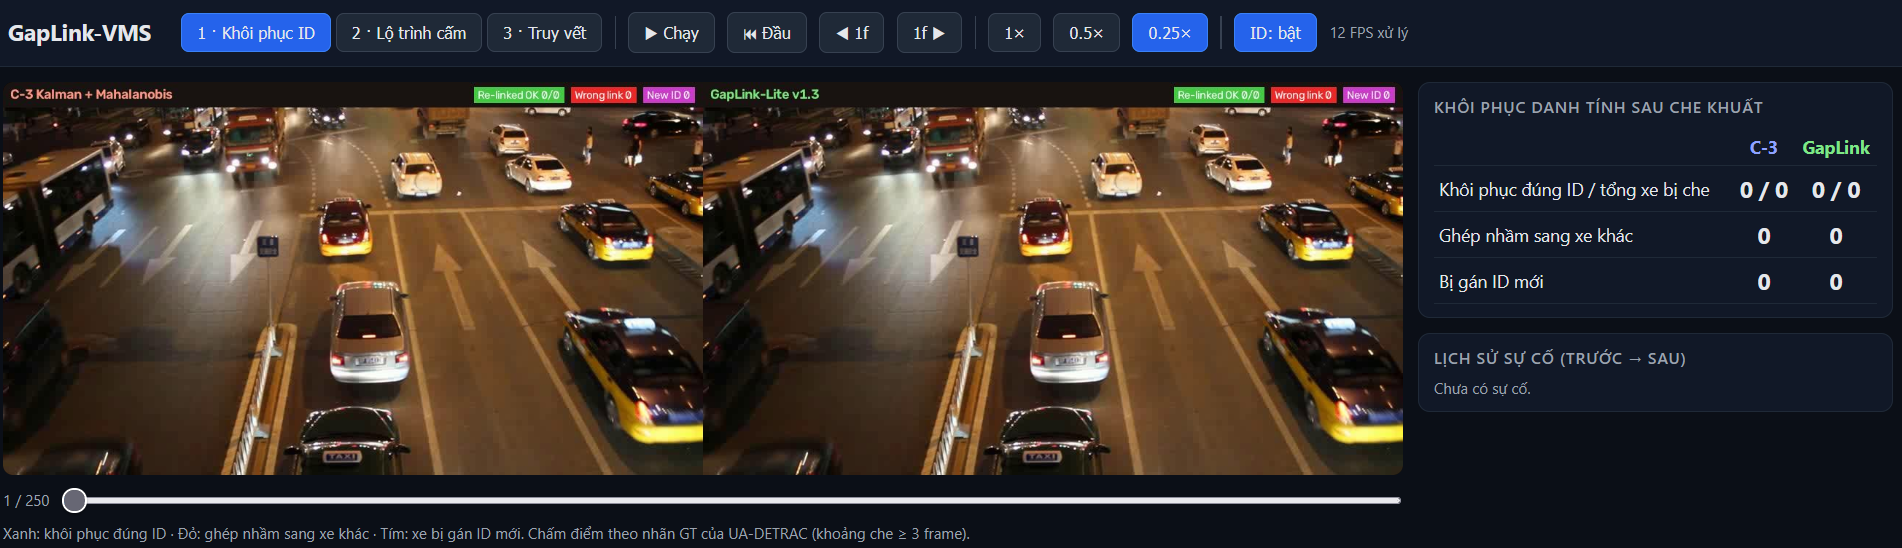
\includegraphics[width=\textwidth]{figures/fig_vms_lite_ui.png}
    \caption{Dashboard GapLink-VMS (clip khôi phục danh tính, khung hình đầu): C-3 Kalman (khung trái) và GapLink-Lite v1.3 (khung phải), thanh công cụ, bảng kết quả và lịch sử sự cố}
    \label{fig:vms_ui}
\end{figure}

Mỗi xe có một box và ID tracker của nó, và màu thể hiện điều đã xảy ra với ID đó, được chấm theo ground truth: xanh lá --- được tái liên kết đúng xe sau che khuất; đỏ --- bị liên kết với một xe khác; tím --- xe xuất hiện lại với ID mới. Trong clip lộ trình, $Z_A$ và $Z_B$ được vẽ trên mặt đường và vi phạm được đóng khung đỏ (đúng ID), hổ phách (sai ID) hoặc tím (vi phạm giả). Trong clip mục tiêu, đường đi quan sát được vẽ bằng nét liền và, khi mục tiêu bị che, box và đường đi dự đoán được vẽ bằng nét đứt. Mỗi khung có bộ đếm riêng, nên có thể so sánh hai phương pháp ở bất kỳ khung hình nào (Hình~\ref{fig:vms_clips}).

\begin{figure}[H]
    \centering
    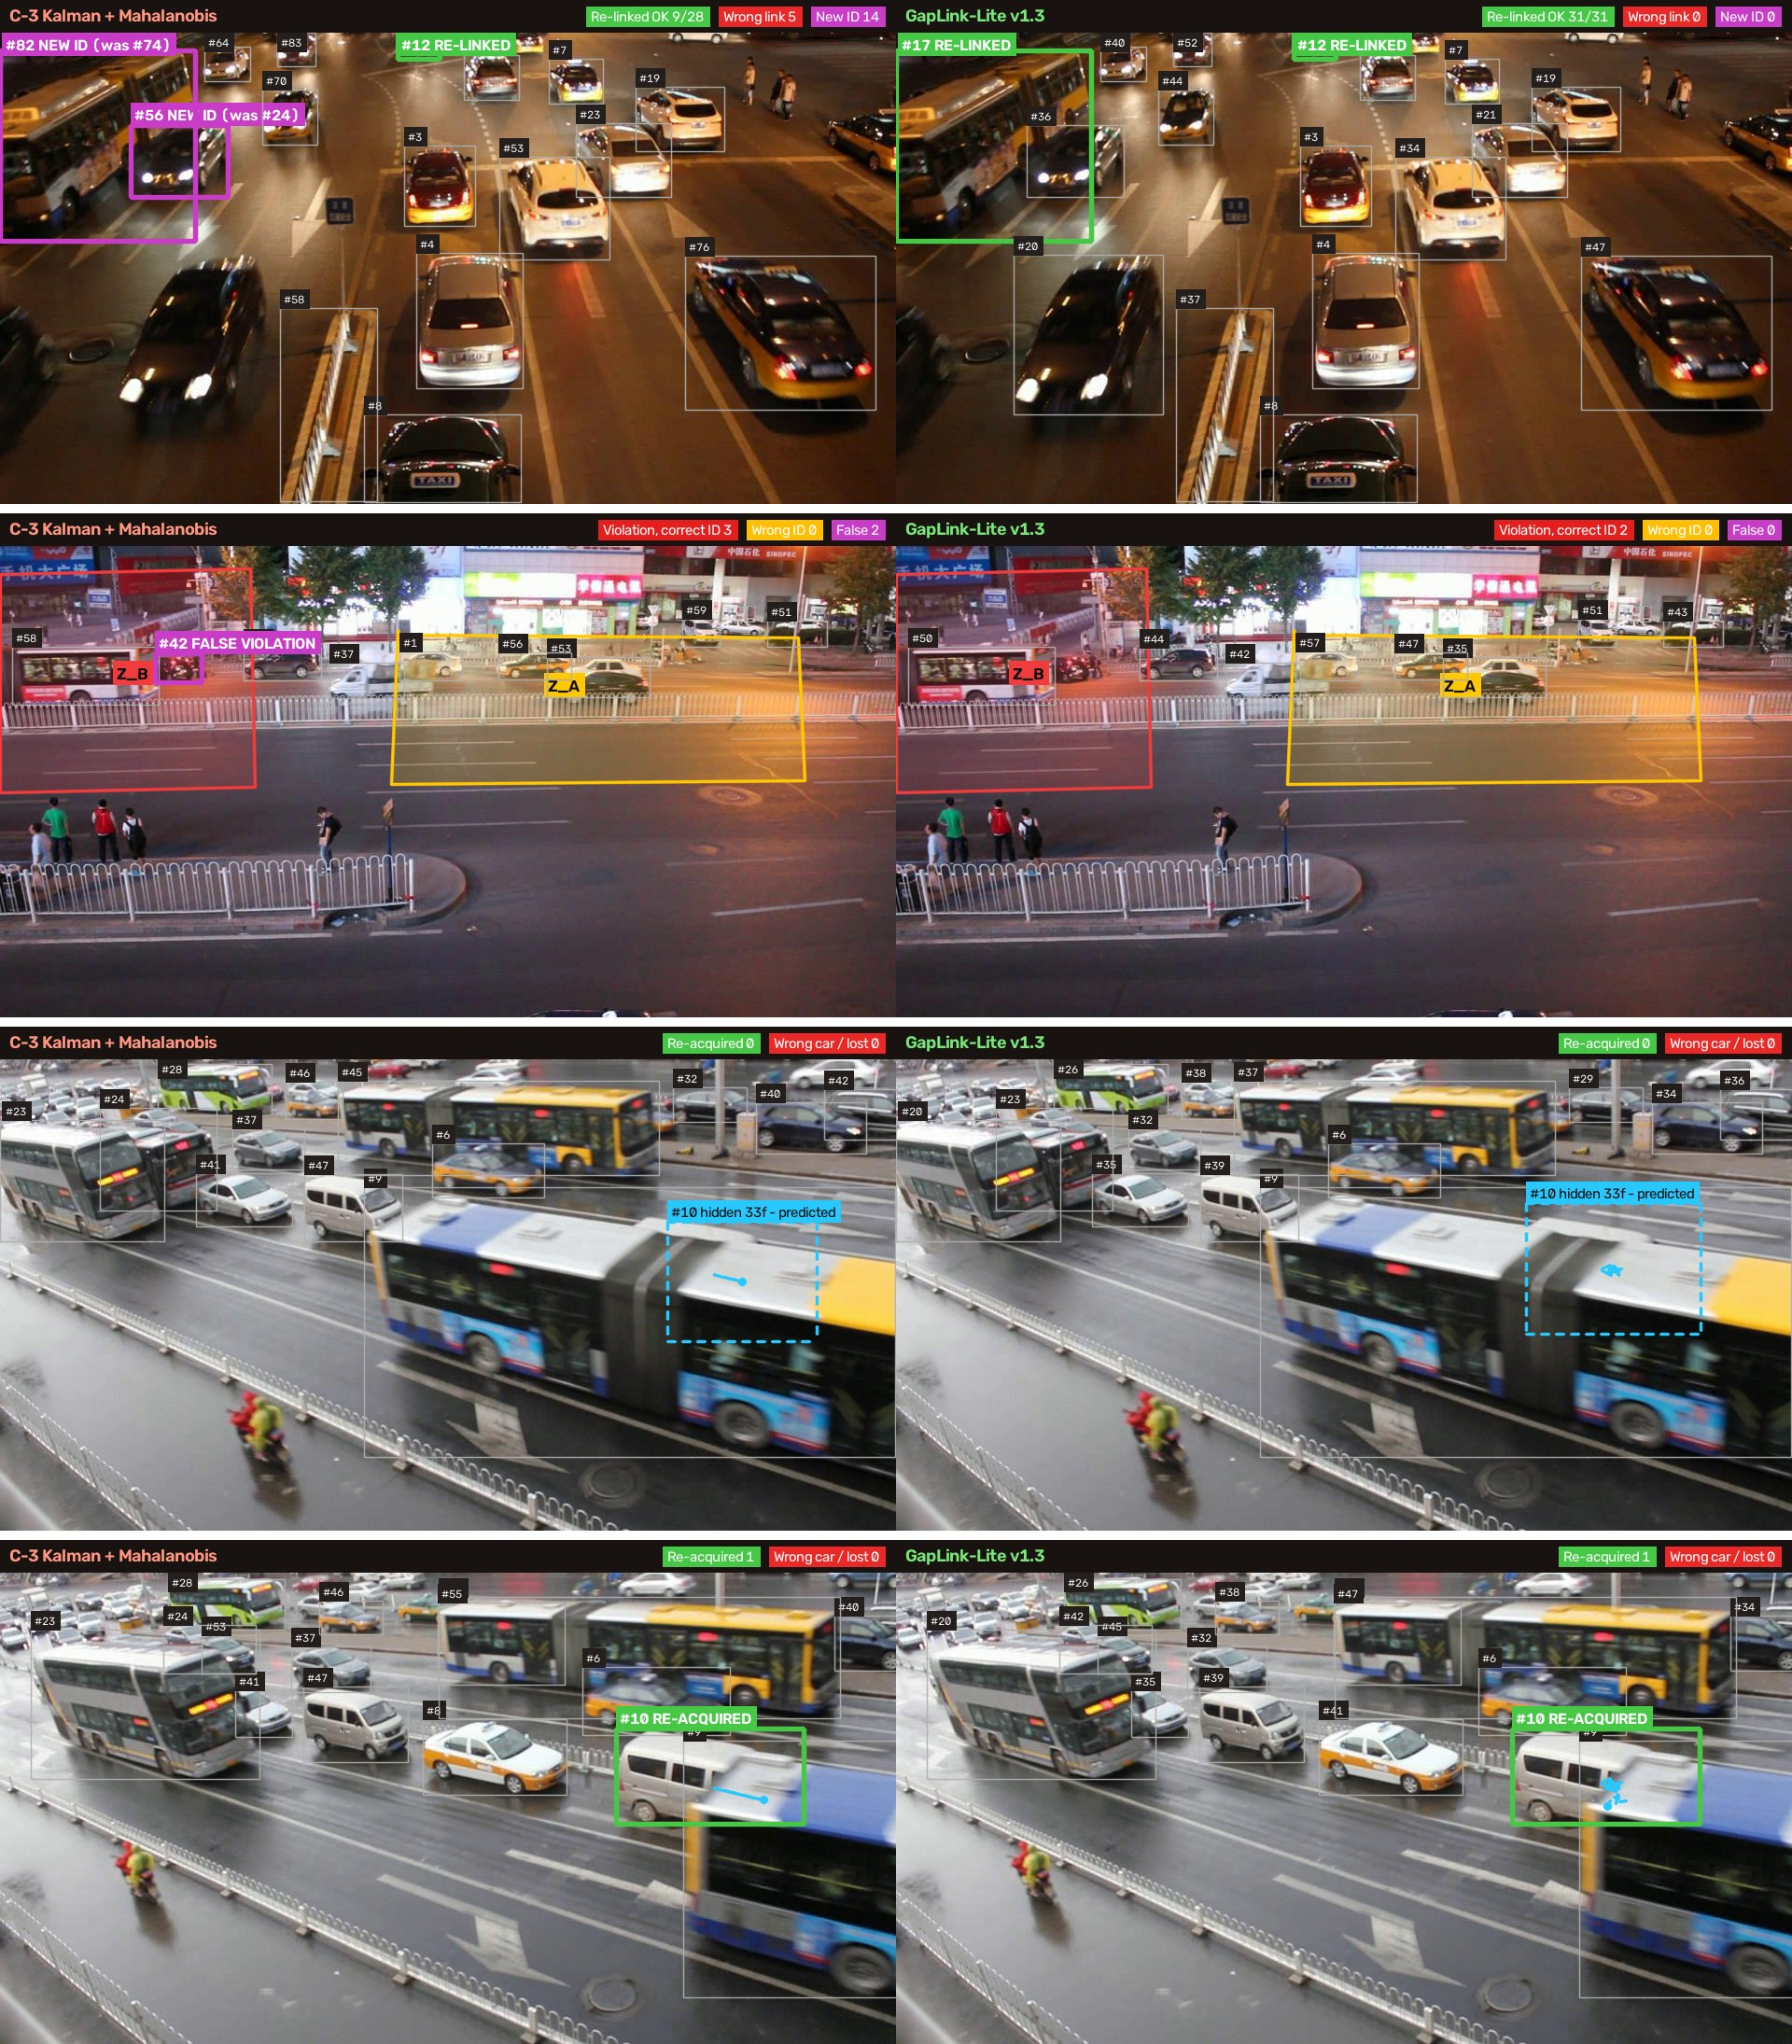
\includegraphics[width=\textwidth]{figures/fig_vms_clips.jpg}
    \caption{Đầu ra của bảng điều khiển trên ba clip (khung trái C-3, khung phải GapLink-Lite v1.3). Từ trên xuống: clip danh tính, khung 123 --- C-3 gán ID mới (tím) cho các xe bị che mà GapLink-Lite tái liên kết được (xanh lá); clip lộ trình, khung 129 --- C-3 báo một vi phạm giả trong $Z_B$; clip mục tiêu, khung 71 và 96 --- xe van đang khóa bị che sau xe buýt khớp nối (box nét đứt: vị trí dự đoán) và được bắt lại.}
    \label{fig:vms_clips}
\end{figure}

\section{Kiểm thử và Cải tiến}
\label{sec:testing_improvements}

\subsection{Kiểm thử Phần mềm}
\label{sec:software_testing}

Mã nguồn được kiểm tra bằng bộ kiểm thử tự động gồm 71 test (Bảng~\ref{tab:tests}). Các test không cần GPU: chúng bao phủ chuẩn hóa Sinkhorn (biên, bất biến với padding, đồng biến hoán vị, ngân sách tham số), sự đồng nhất của việc xây dựng sự kiện giữa huấn luyện và tracking, chèn che khuất, các độ đo kể cả một ca IDF1 kiểm bằng tay, hiệu chuẩn, bootstrap theo địa điểm, gán nhãn sự kiện detector, đóng băng kết quả, và logic bảng điều khiển (chấm lộ trình, phán quyết tái liên kết, nhãn ID, một lần chạy đầu-cuối trên clip demo). Mọi số liệu báo cáo đều gắn với checkpoint, tập sự kiện và kết quả đã băm, nên có thể tái lập chính xác.

\begin{table}[H]
    \centering
    \caption{Kết quả kiểm thử tự động (71 test, $5.3$~s trên laptop của dự án)}
    \label{tab:tests}
    \small
    \begin{tabularx}{\textwidth}{X c c c}
        \toprule
        \textbf{Nhóm test (file)} & \textbf{Số test} & \textbf{Đạt} & \textbf{Lỗi} \\
        \midrule
        Lõi mô hình: lớp Sinkhorn, hiệu chuẩn & 7 & 7 & 0 \\
        Dữ liệu và sự kiện: chuyển đổi, chia tập, lấy mẫu sự kiện, parity, chèn che khuất & 7 & 7 & 0 \\
        Tracking và độ đo: tracker, IDF1, bootstrap theo địa điểm, phân tích lỗi & 10 & 10 & 0 \\
        Đánh giá trực tiếp: sự kiện detector, chọn điểm vận hành, gating & 14 & 14 & 0 \\
        Tái lập: manifest đóng băng & 4 & 4 & 0 \\
        Bảng điều khiển: quy tắc an ninh, profile, metadata clip, render, nhãn ID, phán quyết tái liên kết, chạy đầu-cuối & 25 & 25 & 0 \\
        Công cụ thăm dò ngoài miền & 4 & 4 & 0 \\
        \midrule
        \textbf{Tổng} & \textbf{71} & \textbf{71} & \textbf{0} \\
        \bottomrule
    \end{tabularx}
\end{table}

\subsection{Đánh giá Thực nghiệm}
\label{sec:experimental_evaluation}

Bảng~\ref{tab:eval_vs_target} so sánh kết quả cuối cùng với các mục tiêu cố định từ trước: các giả thuyết đăng ký trước cho Giai đoạn~1, mục tiêu $5\%$ liên kết sai và tốc độ thời gian thực cho Giai đoạn~2.

\begin{table}[H]
    \centering
    \caption{Kết quả đánh giá so với mục tiêu}
    \label{tab:eval_vs_target}
    \small
    \begin{tabularx}{\textwidth}{>{\raggedright\arraybackslash}p{3.9cm} >{\raggedright\arraybackslash}X l l}
        \toprule
        \textbf{Tiêu chí} & \textbf{Kết quả} & \textbf{Mục tiêu} & \textbf{Trạng thái} \\
        \midrule
        H1: mức tăng Top-1 trên tập khó so với baseline tốt nhất & $+7.33$~pp $[6.13, 8.77]$ & $\ge 3.0$~pp & Được ủng hộ \\
        H2: độ phủ 90\% sau hiệu chuẩn, 3 nhóm khoảng trống (val.) & $87.71 / 87.64 / 95.14\%$ & $[85, 95]\%$ & Không được ủng hộ \\
        H3: IRR tracker $>$ C-2, C-3 với $\Delta$WLR $\le 0.5$~pp & 3/3 nhóm; IRR $96.20\%$, WLR $0.21\%$ & $\ge 2/3$ nhóm & Được ủng hộ \\
        P1: IRR khi không tái liên kết & $0.00\%$ & $< 5\%$ & Đạt \\
        Kích thước mô hình & $327\,979$ tham số & $< 1$M & Đạt \\
        Nat-WLR trực tiếp (test, v1.3) & $6.09\%$ & $\le 5\%$ & Không đạt \\
        Nat-IRR trực tiếp so với baseline mạnh nhất (C-2) & $84.41$ so với $84.58\%$ & không thấp hơn & Ngang nhau (CI $[-1.33, 1.08]$) \\
        Tốc độ bảng điều khiển (detection cache, mô hình trên CPU) & $36$--$46$ FPS & $\ge 25$ FPS & Đạt \\
        \bottomrule
    \end{tabularx}
\end{table}

\textbf{Các clip trình diễn.} Ba clip được chọn từ video test bằng cách chạy cả hai tracker trên toàn bộ $40$ video test và giữ lại, cho mỗi nhiệm vụ, các cửa sổ mà phán quyết của GapLink-Lite tốt nhất; đây là lựa chọn phục vụ trình diễn, không phải phép đo. Bảng~\ref{tab:demo3} báo cáo số đếm của bảng điều khiển cuối cùng trên mỗi clip.
\begin{itemize}
    \item \textbf{Khôi phục danh tính} ($250$ khung hình một nút giao đông về đêm có xe buýt). GapLink-Lite tái liên kết đúng cả $48$ xe bị che, kể cả xe buýt, trong khi tracker Kalman tái liên kết đúng $21$ trên $51$, liên kết $12$ xe với xe sai và gán ID mới cho $18$ xe; ngay ở khung $98$, C-3 mới đúng $5/21$ so với $27/27$ của GapLink-Lite.
    \item \textbf{Lộ trình cấm} ($250$ khung hình một đường phố về đêm; $Z_A$ và $Z_B$ trên làn đường phía xa). C-3 phát sáu cảnh báo: ba đúng, một sai ID và hai giả --- ở khung $129$, track \#42 tới $Z_B$ dù xe của nó chưa từng ở $Z_A$. GapLink-Lite phát hai cảnh báo, cả hai đều đúng. Clip này thể hiện độ chính xác chứ không phải recall; trên $40$ video test, C-3 bắt được nhiều vi phạm bị che hơn ($47.53\%$ so với $42.59\%$) với tỉ lệ báo động giả cao hơn ba lần.
    \item \textbf{Bám theo mục tiêu} ($156$ khung hình một trục đường mưa). Xe van đang khóa bị che sau xe buýt khớp nối trong $58$ khung hình; cả hai tracker đều bắt lại nó ở khung $96$, nhưng sáu khung sau, sau thêm một khoảng trống ba khung ở mép xe buýt, C-3 để xe van quay lại với ID mới (\#10 thành \#58), nên khóa mất mục tiêu, còn GapLink-Lite giữ xe van với \#10 đến hết clip ($4$ lần bắt lại, không mất mục tiêu).
\end{itemize}

\begin{table}[H]
    \centering
    \caption{Kết quả trên ba clip trình diễn (bảng điều khiển cuối, C-3 so với GapLink-Lite v1.3)}
    \label{tab:demo3}
    \small
    \begin{tabularx}{\textwidth}{l X c c}
        \toprule
        \textbf{Clip (nguồn)} & \textbf{Tiêu chí} & \textbf{C-3 Kalman} & \textbf{GapLink-Lite} \\
        \midrule
        1. Khôi phục danh tính & Tái liên kết đúng / số xe bị che & $21 / 51$ & $\mathbf{48 / 48}$ \\
        (MVI\_40775, 250 khung) & Liên kết sai & $12$ & $\mathbf{0}$ \\
         & Xe bị gán ID mới & $18$ & $\mathbf{0}$ \\
        \midrule
        2. Lộ trình cấm & Vi phạm đúng ID & $3$ & $2$ \\
        (MVI\_40761, 250 khung) & Vi phạm sai ID & $1$ & $\mathbf{0}$ \\
         & Vi phạm giả & $2$ & $\mathbf{0}$ \\
        \midrule
        3. Bám theo mục tiêu & Số lần bắt lại mục tiêu & $1$ & $\mathbf{4}$ \\
        (MVI\_40864, 156 khung) & Mất mục tiêu (đổi ID) & $1$ (khung 102) & $\mathbf{0}$ \\
        \bottomrule
    \end{tabularx}
\end{table}

\textbf{Các cải tiến qua từng vòng.} Ba thay đổi định hình hệ thống cuối cùng. (i) Kiểm tra lại lần chạy test đã khóa đầu tiên phát hiện một lỗi chuyển đổi dữ liệu (vùng bỏ qua bị gộp thành một track giả) và cửa sổ track bị mất ngắn hơn khoảng trống dài nhất; cả hai đều được sửa và mô hình được huấn luyện và đóng băng lại. (ii) Giai đoạn~2 cho thấy mô hình chỉ huấn luyện trên box ground-truth liên kết quá vội trên box detector; fine-tune theo detector (v1.3) giảm một nửa tỉ lệ liên kết sai trực tiếp so với baseline mạnh nhất. (iii) Bảng điều khiển trình diễn được xây lại quanh ba nhiệm vụ và được profile; chạy mô hình nhỏ trên CPU và đơn giản hóa phần vẽ đã nâng tốc độ từ $12$--$14.5$ lên $36$--$46$~FPS.

\subsection{Hạn chế}
\label{sec:limitations}

\begin{itemize}
    \item \textbf{Hiệu chuẩn với khoảng trống dài.} H2 không đạt vì hệ số hiệu chuẩn cho khoảng trống dài, khớp trên bốn địa điểm validation, phủ quá ($95.86\%$ trên test).
    \item \textbf{Liên kết sai khi chạy trực tiếp.} Không phương pháp nào, kể cả GapLink-Lite ($6.09\%$), giữ được tỉ lệ liên kết sai trực tiếp dưới mục tiêu $5\%$ trên test, và so với baseline vận tốc không đổi, lợi thế nằm ở liên kết sai và báo động giả chứ không ở khả năng khôi phục hay recall lộ trình.
    \item \textbf{Lịch sử đánh giá.} Tập test Giai đoạn~1 được đánh giá lần thứ hai sau khi sửa lỗi chuyển đổi dữ liệu, và video test trực tiếp được chấm cho cả checkpoint gốc lẫn checkpoint thích ứng detector; cả hai lần chạy lại đều được báo cáo công khai thay vì thay thế.
    \item \textbf{Phạm vi dữ liệu.} Không có lớp xe máy, camera cố định đặt cao tại các thành phố Trung Quốc, bốn địa điểm validation, $7$ trong $15$ địa điểm test dùng chung với huấn luyện (không có ảnh hưởng đo được: $93.39\%$ so với $93.44\%$ Top-1), và chỉ một seed cho lần fine-tune trực tiếp.
    \item \textbf{Clip trình diễn.} Các clip được chọn trên video test để thể hiện rõ sự khác biệt; số đếm của chúng minh họa hành vi và không phải ước lượng không chệch (bảng Giai đoạn~2 đã đóng băng mới là ước lượng đó).
\end{itemize}
